\section{Stage 1: Benchmark Generator} \label{sec:work_stage1_program_generator}




To use machine learning models to predict energy consumption, it is necessary to have a large amount of data. This data can be obtained by generating benchmarks that are then executed to collect energy profiles. The benchmark generator is responsible for creating these benchmarks, which are then used to train the machine learning models. The generator is designed to be flexible and adaptable, allowing it to generate a wide variety of benchmarks based on different templates and input parameters. The architecture of the benchmark generator can be seen in Figure~\ref{fig:program_generator}.


The benchmark generator works alongside with Java Spoon to make it the more general as possible allowing custom programs to be mass generated.

The generator is capable of generating benchmarks for custom, developer-created, Java classes, as well as for the most common APIs, such as collections interface implementations (Lists, Sets, Maps), and utility classes like Math, Base64, Duration. It can also be configured to analyze all public methods of a class or just specific ones.

\begin{figure}[htbp]%[H]
    \centering
    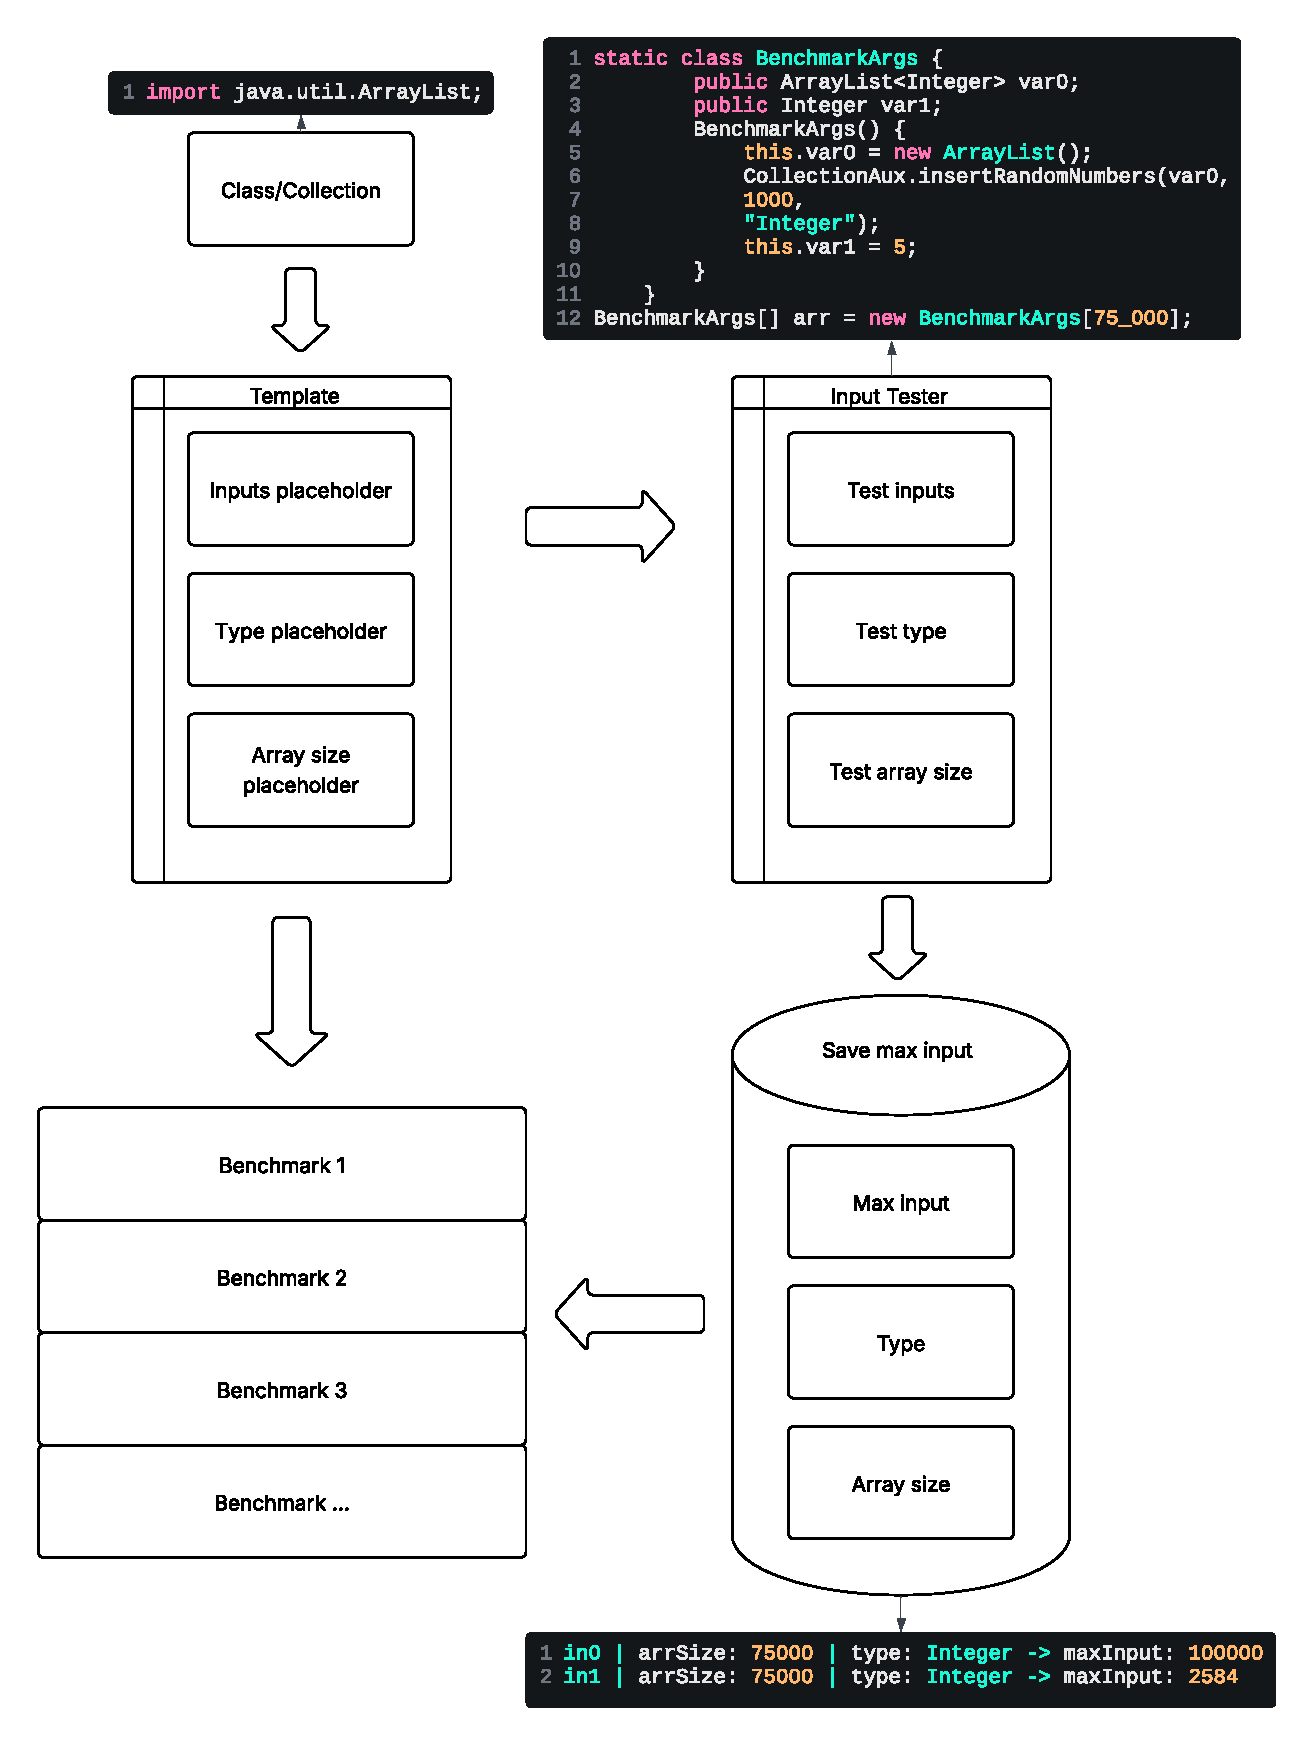
\includegraphics[width = 1 \textwidth]{figures/program_generator.pdf}
    \caption{Benchmark Generator}
    \label{fig:program_generator}
\end{figure}


\subsection{Template Creation} \label{sec:work_stage1_template_creation}

The first step to generate multiple benchmarks is to first create an intermediate template capable of holding the necessary code that will later be used for energy profiling.

To generate benchmarks for a specific class, the user has to input the name of the collection or the name of the custom program it wants to generate. For the collections of Lists, Sets and Maps, the generator is prepared to create more than one implementation of those collections, for example, if the objective is to generate benchmarks to the List collection, the benchmark generator will use the \texttt{ArrayList}, \texttt{LinkedList}, \texttt{Vector} and \texttt{CopyOnWriteArrayList}. The user can also input the name of the method to be analyzed, or simply gather all the available methods in the class, which are then found using Spoon.
After the search for the methods, the generator has access to all the methods it will analyze and their input parameters. 
Since it has access to the whole class, it can see how its constructors are called, and use them if any of the methods parameters requires. 
It recursively calls constructors if needed, making it very versatile to use. After identifying the methods that will be targeted, it starts by creating templates for each of them. The templates are Java classes that contain the necessary code to run the method, and placeholders for the inputs and types. The inputs we consider include the parameters received directly by the method, as well as the values required to construct any objects that are passed as parameters. The templates are structured so that they can be easily modified later, allowing the generator to create multiple benchmarks based on the same template. The templates are designed following the structure below:

\begin{itemize}

\item Input placeholders: Placeholders that will be later changed with real values for inputs, in this case inputs are variable values. 

\item Type placeholder: Placeholders that will later be replaced with Java wrapper classes.
  
\item Array Size placeholder: Placeholder that will later be replaced with the value of an array size. (more details in~\ref{sec:work_stage2_orchestrator}). 

\end{itemize}

Also, the template is structured so that the benchmarks will work in harmony with the \textbf{Orchestrator}, that will extract the energy profile for each benchmark (see Section~\ref{sec:work_stage2_orchestrator}), so when the placeholders are replaced with actual values, the orchestrator can run the program, and communicate with them.


\begin{listing}[htbp]
\noindent\rule{\linewidth}{0.4pt}
\begin{minted}[linenos, fontsize=\small, frame=none, bgcolor=white,breaklines=true,breakanywhere=true]{java}
static class BenchmarkArgs {
        public ArrayList<changetypehere> var0;

        public changetypehere var1;

        BenchmarkArgs() {
            this.var0 = new ArrayList();
            CollectionAux.insertRandomNumbers(var0, "ChangeValueHere1_changetypehere", "changetypehere");
            this.var1 = "ChangeValueHere2_changetypehere";
        }
    }
\end{minted}
\noindent\rule{\linewidth}{0.4pt}
\caption{Example of variable placeholders creations}            
\label{lst:var_placeholders}
\end{listing}

Templates will have the definitions of a class that holds the necessary variables that the method under evaluation needs to run. Listing~\ref{lst:var_placeholders} shows an example of template to evaluate the method \texttt{List.add(Object)}. It follows the algorithm described in Algorithm~\ref{alg:template_creation_algorithm}. First it creates the list with the smallest constructor possible, then if the variable is a collection (List, Set, Map), or an array, it calls a custom-made method that populates collections with random values of a given type, and then it starts creating variables of parameters that the method \texttt{List.add(Object)} uses. The placeholder \texttt{ChangeValueHere1} will change to a random number, it contains a number \texttt{1} because it represents the input number of the method that will later help the model training understand how inputs can affect energy consumption. The placeholder \texttt{changetypehere} later changes to a type. The template after the transformation can be seen in the Listing~\ref{lst:var_placeholders_replaced}



\begin{algorithm}[htbp]
\caption{Template Creation Algorithm}
\label{alg:template_creation_algorithm}
\begin{algorithmic}[1]
    \Statex \textbf{Given:}
    \Statex \hspace{\algorithmicindent} $collection \coloneqq \{\text{List}\}$, collection selected.
    \Statex \hspace{\algorithmicindent} $ds \coloneqq \{\text{List, Map, Set, arrays}\}$, existent data structures.
    \Statex \hspace{\algorithmicindent} $methods \coloneqq \{\text{add, size, get}, \dots\}$, the set of methods of the classes.

    \Procedure{CreateTemplate}{}
        \State \textit{methods} $\gets$ \Call{getMethods}{\texttt{collection}}
        \ForAll{method \textbf{in} methods}
            \State vars $\gets$ empty list
            \ForAll{parameter \textbf{in} \texttt{method.parameters}}
                \State \textit{var} $\gets$ \Call{ParameterCreation}{\texttt{parameter.type}}
                \If{$parameter.type \in ds$}
                    \State \Call{FillWithRandomValues}{var, maxSizePlaceHolder, typePlaceHolder}
                \EndIf
                \State Append var to vars
            \EndFor
            \State \Call{CreateBenchmarkArrayMethod}{method, vars}
            \State \Call{CreateBenchmarkMethod}{method, vars}
            \State \Call{CreateOrchestratorStartSetup}{}
            \State \Call{CreateComputationMethod}{method, vars}
            \State \Call{CreateOrchestratorEndSetup}{}
            \State \Call{SaveTemplate}{}
        \EndFor
    \EndProcedure

    \Procedure{ParameterCreation}{\textit{type}}
        \If{\Call{IsPrimitive}{type}}
            \State \Return type
        \Else
            \State dependencies $\gets$ \Call{GetConstructorArguments}{type}
            \State args $\gets$ empty list
            \ForAll{dep \textbf{in} dependencies}
                \State arg $\gets$ \Call{ParameterCreation}{dep}
                \State Append arg to args
            \EndFor
            \State instance $\gets$ \Call{Instantiate}{type, args} \Comment{Create an instance, using the smallest constructor.}
            \State \Return instance
        \EndIf
    \EndProcedure
\end{algorithmic}
\end{algorithm}



\begin{listing}[htbp]
\noindent\rule{\linewidth}{0.4pt}
\begin{minted}[linenos, fontsize=\small, frame=none, bgcolor=white,breaklines=true,breakanywhere=true]{java}
static class BenchmarkArgs {
        public ArrayList<Integer> var0;

        public Integer var1;

        BenchmarkArgs() {
            this.var0 = new ArrayList();
            CollectionAux.insertRandomNumbers(var0, 1000, "Integer");
            this.var1 = 10;
        }
    }
\end{minted}
\noindent\rule{\linewidth}{0.4pt}
\caption{Example of variable placeholders replaced}            
\label{lst:var_placeholders_replaced}
\end{listing}



It is worth mentioning that the types used by the generator are the Java wrapper classes, which are object representations of the primitive types. Using these types it is possible to achieve a more general generator, as every program can use them and if other custom types were used it would make the generator more complex and not general. Building on this idea, type placeholders are only generated for parameters that can accept multiple types. For example, if a method accepts a parameter of type \texttt{Object} or \texttt{ArrayList<T>}, the generator can substitute a variety of types, \texttt{Object} may become \texttt{Integer} or \texttt{Double}, and \texttt{ArrayList<T>} can be transformed as \texttt{ArrayList<Integer>}, \texttt{ArrayList<Double>}, or any other wrapper type. In contrast, if a method expects a fixed type like \texttt{int}, no type placeholder is generated, as introducing one would result in a semantic error due to incompatible types.

What mostly differs from template to template is the number of variables used, because different methods have different parameters, so the template can have more or less input placeholders, also the type placeholder changes according to the methods types and parameters.


Creating the template for each method allows cutting off time of the benchmark generation by only having to replace values of the placeholders instead of needing to create the whole benchmark all over again, since the benchmarks for the same method only differ in inputs, types and array size, maintaining all the structure.

\subsection{Input Tester} \label{sec:work_stage1_input_tester}

An important aspect of the benchmark generator are the inputs it generates. Every method has its on funcionality that may be dependent on the input values. To be able to better generalize, it is important to find the method input values upper limit. Knowing the maximum size that different parameters can have is fundamental as it needs to be representative, so the energy profiles can cover more cases, but not to large so that the benchmarks start to run out of memory or taking too much time to complete.
The limit definition works by using binary search. It has an inital threshold on the inputs (e.g., 1-100,000 to numerical values) and it starts by trying to run the benchmark with the half of the maximum upper limit threshold (e.g., 50,000). 

It can be important, for pratical reasons, to impose a threashold on the execution time (in this project, we established the threshold as 10 seconds based on empirical experimentation). If the benchmark runs successfully, it will increase the input by half, and if it fails, it will decrease the input by half. This process continues until the maximum value for the input is found.

If the method that is being tested has more than one input, the input tester is responsible to find the upper limit for each parameter individually. First it sets all the input values to 1 and then starts the binary search individually for each of the parameters one by one while leaving the other parameters with the value of 1. Although this is a simplification, this method avoids having to find multiple combinations of parameters which would increase the time complexity exponentially. More robust solutions (such as using a combinatory search) could be implemented in the future. Nevertheless, even using the simplified solution, the process of finding the max inputs is time-consuming. To improve its performance, when the maximum value is found, the values of the input type, maximum value and order (e.g., first, second or third parameter), are stored in a file. This makes subsequent executions much faster. It is worthy to mention that the maximum inputs found depend heavily on the machine where the benchmark generation is taking place, as different hardware will change the maximum values allowed for the inputs. Example 1 illustrates how the input tester works for the method \texttt{List.add(index, Element)}.

\begin{tcolorbox}[
    title=Example 1: Input Testing Process for \texttt{List.add(index, Element)},
    colback=gray!5!white,
    colframe=gray!75!black,
    fonttitle=\bfseries,
    breakable,
    label={box:add-method-testing}
]

Consider analyzing the \texttt{add} method of a list with the following parameters:
\begin{itemize}
    \item \texttt{arg0}: Size of the list (integer)
    \item \texttt{arg1}: Index at which to insert the new value (integer)
    \item \texttt{arg2}: Value to be added (integer)
\end{itemize}

\textbf{Step 1 – Varying \texttt{arg0} (list size):}

\begin{itemize}
    \item Iteration 1: \texttt{arg0 = 25,000}, \texttt{arg1 = 1}, \texttt{arg2 = 1}
    \item Iteration 2: \texttt{arg0 = 12,500}, \texttt{arg1 = 1}, \texttt{arg2 = 1}
    \item Iteration 3: \texttt{arg0 = 6,250}, \texttt{arg1 = 1}, \texttt{arg2 = 1}
    \item $\vdots$
    \item Final Iteration: \texttt{arg0 = 1,700}, \texttt{arg1 = 1}, \texttt{arg2 = 1}
\end{itemize}

\textbf{Step 2 – Varying \texttt{arg1} (index):}

\begin{itemize}
    \item Iteration 1: \texttt{arg0 = 1}, \texttt{arg1 = 25,000}, \texttt{arg2 = 1}
    \item Iteration 2: \texttt{arg0 = 1}, \texttt{arg1 = 12,500}, \texttt{arg2 = 1}
    \item $\vdots$
    \item Final Iteration: \texttt{arg0 = 1}, \texttt{arg1 = 1}, \texttt{arg2 = 1}
\end{itemize}

{Note: Since the list size (\texttt{arg0}) remains 1, the maximum valid index (\texttt{arg1}) is constrained to 1. This reveals a limitation in the input testing approach.}

\textbf{Step 3 – Varying \texttt{arg2} (value to be added):}

\begin{itemize}
    \item Iteration 1: \texttt{arg0 = 1}, \texttt{arg1 = 1}, \texttt{arg2 = 25,000}
    \item Iteration 2: \texttt{arg0 = 1}, \texttt{arg1 = 1}, \texttt{arg2 = 37,500}
    \item $\vdots$
    \item Final Iteration: \texttt{arg0 = 1}, \texttt{arg1 = 1}, \texttt{arg2 = 100,000}
\end{itemize}

\textbf{Final stored input limits:}
\begin{itemize}
    \item \texttt{arg0} — \texttt{integer} — \texttt{1,700}
    \item \texttt{arg1} — \texttt{integer} — \texttt{1}
    \item \texttt{arg2} — \texttt{integer} — \texttt{100,000}
\end{itemize}

\end{tcolorbox}


The fact that the input has a pre-determined range it allows using binary search which makes the search much faster than linear search.
Nevertheless, the input search does not come without some limitations. First it is constrained to identifying valid input values within the range. As an example, throughout this project we dealt frequently with lists and collections, which require a minimum size of 1 to function correctly. Although this value can be changed in the future, for now it ensures compatibility with most common data structures. The higher bound was chosen due to empirical evidences, as larger input values would lead to limitating execution times and memory crashes. Another constraint is on how the input handles multiple parameter methods. During its search for a valid input, it needs to fix all the other parameters that is not searching, with a default value (typically the lower bound). This approach simplifies the testing process and improves efficiency by avoiding the exponential complexity of testing all possible parameter combinations. However, it will introduce limitations in cases where the parameters are interdependent, which can lead to not estimating the real highest input possible. 
Despite these limitations, the input search plays a crucial role in ensuring that the benchmark generator produces viable test cases. By identifying input ranges that are both valid and computationally achievable, it reduces the unusable generated benchmarks (e.g., due to timeouts or crashes), and maximizing the number of generated benchmarks, that can be used for energy profiling.



\subsection{Benchmark Generation} \label{sec:work_stage1_program_generation}

Finally, when the templates are created, and the maximum inputs are found the benchmark generation can finally begin. This part consists on picking every template created and replacing the placeholder values with actual values created by a random number generator. It follows the algorithm described in Algorithm~\ref{alg:template_fullfillment_algorithm}

It starts by looping through the types and changing them to the Java wrapper classes, then it loops through the array size. Lastly, it loops through the input sizes determined by the input tester and can repeat this process a configurable number of times. By increasing the number of iterations, results in more benchmarks being generated with random inputs, constrained by the previously identified input bounds. 




\begin{algorithm}[htbp]
\caption{Template Fullfillment Algorithm}
\label{alg:template_fullfillment_algorithm}
\begin{algorithmic}[1]
    \Statex \textbf{Given:}
    \Statex \hspace{\algorithmicindent} $templates$, list of templates previously generated.
    \Statex \hspace{\algorithmicindent} $types \coloneqq \{\text{Integer, Double, Long, Float, Short, Character }\}$, types to be replaced.
    \Statex \hspace{\algorithmicindent} $arraySize \coloneqq \{\text{75\,000, 100\,000, 150\,000}\}$, array sizes to be used.
    \Statex \hspace{\algorithmicindent} $template.maxInputs $, each template has a maximum input file associated to it.
    \Statex \hspace{\algorithmicindent} $iterations $, number of iterations for the input loop.

\Procedure{FullfillTemplate}{}
    \ForAll{template \textbf{in} templates}
        \ForAll{type \textbf{in} \texttt{types}}
            \State program $\gets$ \Call{Replace}{template, "typePlaceHolder", type}
                \ForAll{arraySize \textbf{in} \texttt{arraySizes}}
                    \State program2 $\gets$ \Call{Replace}{program, "arraySizePlaceHolder", arraySize}
                        \For{$i \gets 0$ \textbf{to} \texttt{iterations}}
                            \State program3 $\gets$ \Call{replaceValues}{program2, template.maxInputs}
                            \State \Call{SaveToFile}{program3}
                        \EndFor
                \EndFor
        \EndFor
    \EndFor
    
\EndProcedure

\vspace{1em} 

\Procedure{ReplaceValues}{program, maxInputs}
    \State valuesToReplace $\gets$ \Call{FindStringsToReplace}{program, placeholderPattern}
    \For{$i \gets 0$ \textbf{to} \Call{Size}{valuesToReplace} - 1}
        \State value $\gets$ valuesToReplace[i]
        \State type $\gets$ \Call{ExtractType}{value}
        \State max $\gets$ maxInputs[i]
        \State min $\gets$ \Call{Min}{1, max}
        \State newValue $\gets$ \Call{GetRandomValue}{type, min, max}
        \State program $\gets$ \Call{Replace}{program, value, newValue}
    \EndFor
    \State \Return program
\EndProcedure

\end{algorithmic}
\end{algorithm}

This process easily generate thousands of benchmarks which are crucial to train machine learn models that are able to predict energy consumption. When generating benchmarks, a number is chosen to balance the requirements for effective model training while minimizing the time spent on input testing and collecting energy profiles. Afterwards, that the benchmarks are ready to be compiled and used.